\documentclass[1p]{elsarticle_modified}
%\bibliographystyle{elsarticle-num}

%\usepackage[colorlinks]{hyperref}
%\usepackage{abbrmath_seonhwa} %\Abb, \Ascr, \Acal ,\Abf, \Afrak
\usepackage{amsfonts}
\usepackage{amssymb}
\usepackage{amsmath}
\usepackage{amsthm}
\usepackage{scalefnt}
\usepackage{amsbsy}
\usepackage{kotex}
\usepackage{caption}
\usepackage{subfig}
\usepackage{color}
\usepackage{graphicx}
\usepackage{xcolor} %% white, black, red, green, blue, cyan, magenta, yellow
\usepackage{float}
\usepackage{setspace}
\usepackage{hyperref}

\usepackage{tikz}
\usetikzlibrary{arrows}

\usepackage{multirow}
\usepackage{array} % fixed length table
\usepackage{hhline}

%%%%%%%%%%%%%%%%%%%%%
\makeatletter
\renewcommand*\env@matrix[1][\arraystretch]{%
	\edef\arraystretch{#1}%
	\hskip -\arraycolsep
	\let\@ifnextchar\new@ifnextchar
	\array{*\c@MaxMatrixCols c}}
\makeatother %https://tex.stackexchange.com/questions/14071/how-can-i-increase-the-line-spacing-in-a-matrix
%%%%%%%%%%%%%%%

\usepackage[normalem]{ulem}

\newcommand{\msout}[1]{\ifmmode\text{\sout{\ensuremath{#1}}}\else\sout{#1}\fi}
%SOURCE: \msout is \stkout macro in https://tex.stackexchange.com/questions/20609/strikeout-in-math-mode

\newcommand{\cancel}[1]{
	\ifmmode
	{\color{red}\msout{#1}}
	\else
	{\color{red}\sout{#1}}
	\fi
}

\newcommand{\add}[1]{
	{\color{blue}\uwave{#1}}
}

\newcommand{\replace}[2]{
	\ifmmode
	{\color{red}\msout{#1}}{\color{blue}\uwave{#2}}
	\else
	{\color{red}\sout{#1}}{\color{blue}\uwave{#2}}
	\fi
}

\newcommand{\Sol}{\mathcal{S}} %segment
\newcommand{\D}{D} %diagram
\newcommand{\A}{\mathcal{A}} %arc


%%%%%%%%%%%%%%%%%%%%%%%%%%%%%5 test

\def\sl{\operatorname{\textup{SL}}(2,\Cbb)}
\def\psl{\operatorname{\textup{PSL}}(2,\Cbb)}
\def\quan{\mkern 1mu \triangleright \mkern 1mu}

\theoremstyle{definition}
\newtheorem{thm}{Theorem}[section]
\newtheorem{prop}[thm]{Proposition}
\newtheorem{lem}[thm]{Lemma}
\newtheorem{ques}[thm]{Question}
\newtheorem{cor}[thm]{Corollary}
\newtheorem{defn}[thm]{Definition}
\newtheorem{exam}[thm]{Example}
\newtheorem{rmk}[thm]{Remark}
\newtheorem{alg}[thm]{Algorithm}

\newcommand{\I}{\sqrt{-1}}
\begin{document}

%\begin{frontmatter}
%
%\title{Boundary parabolic representations of knots up to 8 crossings}
%
%%% Group authors per affiliation:
%\author{Yunhi Cho} 
%\address{Department of Mathematics, University of Seoul, Seoul, Korea}
%\ead{yhcho@uos.ac.kr}
%
%
%\author{Seonhwa Kim} %\fnref{s_kim}}
%\address{Center for Geometry and Physics, Institute for Basic Science, Pohang, 37673, Korea}
%\ead{ryeona17@ibs.re.kr}
%
%\author{Hyuk Kim}
%\address{Department of Mathematical Sciences, Seoul National University, Seoul 08826, Korea}
%\ead{hyukkim@snu.ac.kr}
%
%\author{Seokbeom Yoon}
%\address{Department of Mathematical Sciences, Seoul National University, Seoul, 08826,  Korea}
%\ead{sbyoon15@snu.ac.kr}
%
%\begin{abstract}
%We find all boundary parabolic representation of knots up to 8 crossings.
%
%\end{abstract}
%\begin{keyword}
%    \MSC[2010] 57M25 
%\end{keyword}
%
%\end{frontmatter}

%\linenumbers
%\tableofcontents
%
\newcommand\colored[1]{\textcolor{white}{\rule[-0.35ex]{0.8em}{1.4ex}}\kern-0.8em\color{red} #1}%
%\newcommand\colored[1]{\textcolor{white}{ #1}\kern-2.17ex	\textcolor{white}{ #1}\kern-1.81ex	\textcolor{white}{ #1}\kern-2.15ex\color{red}#1	}

{\Large $\underline{12a_{0041}~(K12a_{0041})}$}

\setlength{\tabcolsep}{10pt}
\renewcommand{\arraystretch}{1.6}
\vspace{1cm}\begin{tabular}{m{100pt}>{\centering\arraybackslash}m{274pt}}
\multirow{5}{120pt}{
	\centering
	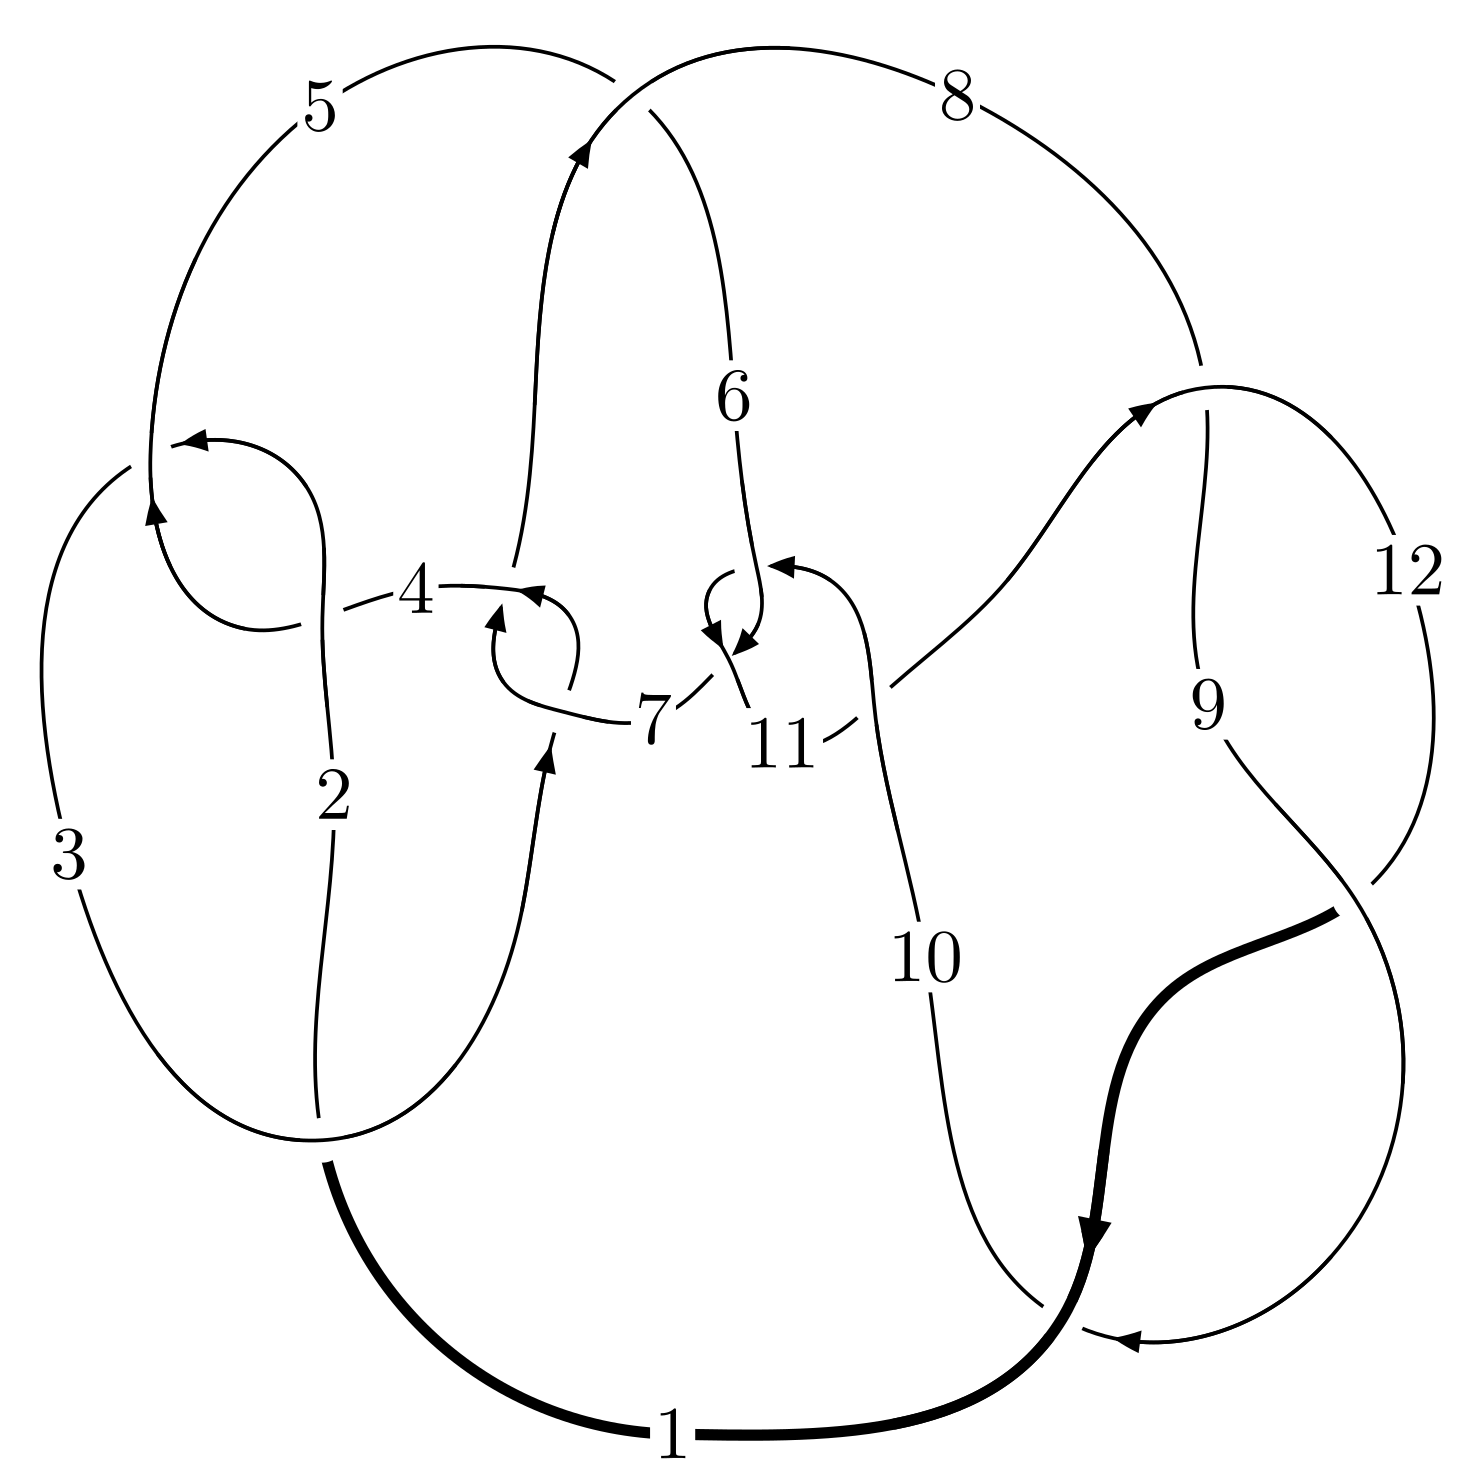
\includegraphics[width=112pt]{../../../GIT/diagram.site/Diagrams/png/842_12a_0041.png}\\
\ \ \ A knot diagram\footnotemark}&
\allowdisplaybreaks
\textbf{Linearized knot diagam} \\
\cline{2-2}
 &
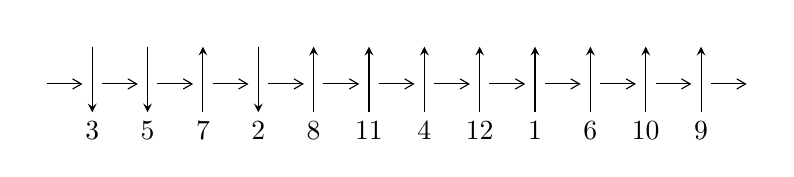
\begin{tikzpicture}[x=20pt, y=17pt]
	% nodes
	\node (C0) at (0, 0) {};
	\node (C1) at (1, 0) {};
	\node (C1U) at (1, +1) {};
	\node (C1D) at (1, -1) {3};

	\node (C2) at (2, 0) {};
	\node (C2U) at (2, +1) {};
	\node (C2D) at (2, -1) {5};

	\node (C3) at (3, 0) {};
	\node (C3U) at (3, +1) {};
	\node (C3D) at (3, -1) {7};

	\node (C4) at (4, 0) {};
	\node (C4U) at (4, +1) {};
	\node (C4D) at (4, -1) {2};

	\node (C5) at (5, 0) {};
	\node (C5U) at (5, +1) {};
	\node (C5D) at (5, -1) {8};

	\node (C6) at (6, 0) {};
	\node (C6U) at (6, +1) {};
	\node (C6D) at (6, -1) {11};

	\node (C7) at (7, 0) {};
	\node (C7U) at (7, +1) {};
	\node (C7D) at (7, -1) {4};

	\node (C8) at (8, 0) {};
	\node (C8U) at (8, +1) {};
	\node (C8D) at (8, -1) {12};

	\node (C9) at (9, 0) {};
	\node (C9U) at (9, +1) {};
	\node (C9D) at (9, -1) {1};

	\node (C10) at (10, 0) {};
	\node (C10U) at (10, +1) {};
	\node (C10D) at (10, -1) {6};

	\node (C11) at (11, 0) {};
	\node (C11U) at (11, +1) {};
	\node (C11D) at (11, -1) {10};

	\node (C12) at (12, 0) {};
	\node (C12U) at (12, +1) {};
	\node (C12D) at (12, -1) {9};
	\node (C13) at (13, 0) {};

	% arrows
	\draw[->,>={angle 60}]
	(C0) edge (C1) (C1) edge (C2) (C2) edge (C3) (C3) edge (C4) (C4) edge (C5) (C5) edge (C6) (C6) edge (C7) (C7) edge (C8) (C8) edge (C9) (C9) edge (C10) (C10) edge (C11) (C11) edge (C12) (C12) edge (C13) ;	\draw[->,>=stealth]
	(C1U) edge (C1D) (C2U) edge (C2D) (C3D) edge (C3U) (C4U) edge (C4D) (C5D) edge (C5U) (C6D) edge (C6U) (C7D) edge (C7U) (C8D) edge (C8U) (C9D) edge (C9U) (C10D) edge (C10U) (C11D) edge (C11U) (C12D) edge (C12U) ;
	\end{tikzpicture} \\
\hhline{~~} \\& 
\textbf{Solving Sequence} \\ \cline{2-2} 
 &
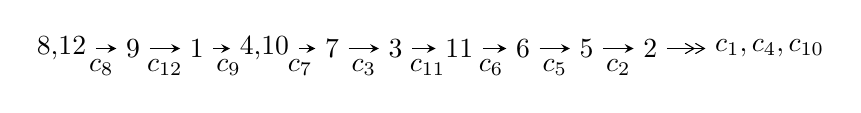
\begin{tikzpicture}[x=23pt, y=7pt]
	% node
	\node (A0) at (-1/8, 0) {8,12};
	\node (A1) at (1, 0) {9};
	\node (A2) at (2, 0) {1};
	\node (A3) at (49/16, 0) {4,10};
	\node (A4) at (33/8, 0) {7};
	\node (A5) at (41/8, 0) {3};
	\node (A6) at (49/8, 0) {11};
	\node (A7) at (57/8, 0) {6};
	\node (A8) at (65/8, 0) {5};
	\node (A9) at (73/8, 0) {2};
	\node (C1) at (1/2, -1) {$c_{8}$};
	\node (C2) at (3/2, -1) {$c_{12}$};
	\node (C3) at (5/2, -1) {$c_{9}$};
	\node (C4) at (29/8, -1) {$c_{7}$};
	\node (C5) at (37/8, -1) {$c_{3}$};
	\node (C6) at (45/8, -1) {$c_{11}$};
	\node (C7) at (53/8, -1) {$c_{6}$};
	\node (C8) at (61/8, -1) {$c_{5}$};
	\node (C9) at (69/8, -1) {$c_{2}$};
	\node (A10) at (11, 0) {$c_{1},c_{4},c_{10}$};

	% edge
	\draw[->,>=stealth]	
	(A0) edge (A1) (A1) edge (A2) (A2) edge (A3) (A3) edge (A4) (A4) edge (A5) (A5) edge (A6) (A6) edge (A7) (A7) edge (A8) (A8) edge (A9) ;
	\draw[->>,>={angle 60}]	
	(A9) edge (A10);
\end{tikzpicture} \\ 

\end{tabular} \\

\footnotetext{
The image of knot diagram is generated by the software ``\textbf{Draw programme}" developed by Andrew Bartholomew(\url{http://www.layer8.co.uk/maths/draw/index.htm\#Running-draw}), where we modified some parts for our purpose(\url{https://github.com/CATsTAILs/LinksPainter}).
}\phantom \\ \newline 
\centering \textbf{Ideals for irreducible components\footnotemark of $X_{\text{par}}$} 
 
\begin{align*}
I^u_{1}&=\langle 
-1.44805\times10^{35} u^{105}+9.77658\times10^{35} u^{104}+\cdots+1.67026\times10^{34} b+1.04667\times10^{35},\\
\phantom{I^u_{1}}&\phantom{= \langle  }-3.36641\times10^{36} u^{105}+2.29468\times10^{37} u^{104}+\cdots+1.67026\times10^{34} a+2.84093\times10^{36},\\
\phantom{I^u_{1}}&\phantom{= \langle  }u^{106}-8 u^{105}+\cdots-8 u+1\rangle \\
I^u_{2}&=\langle 
b,\;u^7-2 u^6-2 u^5+4 u^4+2 u^3- u^2+a- u-3,\;u^8- u^7-3 u^6+2 u^5+3 u^4-2 u-1\rangle \\
I^u_{3}&=\langle 
- a^5+a^4-2 a^2+b+a+1,\;a^6- a^5+2 a^3- a^2- a+1,\;u+1\rangle \\
\\
\end{align*}
\raggedright * 3 irreducible components of $\dim_{\mathbb{C}}=0$, with total 120 representations.\\
\footnotetext{All coefficients of polynomials are rational numbers. But the coefficients are sometimes approximated in decimal forms when there is not enough margin.}
\newpage
\renewcommand{\arraystretch}{1}
\centering \section*{I. $I^u_{1}= \langle -1.45\times10^{35} u^{105}+9.78\times10^{35} u^{104}+\cdots+1.67\times10^{34} b+1.05\times10^{35},\;-3.37\times10^{36} u^{105}+2.29\times10^{37} u^{104}+\cdots+1.67\times10^{34} a+2.84\times10^{36},\;u^{106}-8 u^{105}+\cdots-8 u+1 \rangle$}
\flushleft \textbf{(i) Arc colorings}\\
\begin{tabular}{m{7pt} m{180pt} m{7pt} m{180pt} }
\flushright $a_{8}=$&$\begin{pmatrix}1\\0\end{pmatrix}$ \\
\flushright $a_{12}=$&$\begin{pmatrix}0\\u\end{pmatrix}$ \\
\flushright $a_{9}=$&$\begin{pmatrix}1\\- u^2\end{pmatrix}$ \\
\flushright $a_{1}=$&$\begin{pmatrix}u\\- u^3+u\end{pmatrix}$ \\
\flushright $a_{4}=$&$\begin{pmatrix}201.551 u^{105}-1373.85 u^{104}+\cdots+1189.54 u-170.089\\8.66963 u^{105}-58.5334 u^{104}+\cdots+49.7451 u-6.26650\end{pmatrix}$ \\
\flushright $a_{10}=$&$\begin{pmatrix}- u^2+1\\u^4-2 u^2\end{pmatrix}$ \\
\flushright $a_{7}=$&$\begin{pmatrix}-89.0641 u^{105}+593.235 u^{104}+\cdots-494.775 u+66.5949\\144.038 u^{105}-1011.28 u^{104}+\cdots+967.142 u-136.266\end{pmatrix}$ \\
\flushright $a_{3}=$&$\begin{pmatrix}173.819 u^{105}-1206.87 u^{104}+\cdots+1110.50 u-161.594\\68.8034 u^{105}-417.555 u^{104}+\cdots+217.759 u-26.4940\end{pmatrix}$ \\
\flushright $a_{11}=$&$\begin{pmatrix}- u^5+2 u^3- u\\u^7-3 u^5+2 u^3+u\end{pmatrix}$ \\
\flushright $a_{6}=$&$\begin{pmatrix}31.9491 u^{105}-240.754 u^{104}+\cdots+266.507 u-40.0703\\48.9374 u^{105}-391.734 u^{104}+\cdots+508.341 u-73.9905\end{pmatrix}$ \\
\flushright $a_{5}=$&$\begin{pmatrix}-16.9883 u^{105}+150.980 u^{104}+\cdots-241.834 u+33.9202\\48.9374 u^{105}-391.734 u^{104}+\cdots+508.341 u-73.9905\end{pmatrix}$ \\
\flushright $a_{2}=$&$\begin{pmatrix}193.608 u^{105}-1303.08 u^{104}+\cdots+1072.35 u-154.685\\51.6786 u^{105}-376.900 u^{104}+\cdots+402.827 u-56.7005\end{pmatrix}$\\&\end{tabular}
\flushleft \textbf{(ii) Obstruction class $= -1$}\\~\\
\flushleft \textbf{(iii) Cusp Shapes $= 187.107 u^{105}-1299.22 u^{104}+\cdots+1186.54 u-169.352$}\\~\\
\newpage\renewcommand{\arraystretch}{1}
\flushleft \textbf{(iv) u-Polynomials at the component}\newline \\
\begin{tabular}{m{50pt}|m{274pt}}
Crossings & \hspace{64pt}u-Polynomials at each crossing \\
\hline $$\begin{aligned}c_{1}\end{aligned}$$&$\begin{aligned}
&u^{106}+50 u^{105}+\cdots+115 u+1
\end{aligned}$\\
\hline $$\begin{aligned}c_{2},c_{4}\end{aligned}$$&$\begin{aligned}
&u^{106}-10 u^{105}+\cdots-11 u+1
\end{aligned}$\\
\hline $$\begin{aligned}c_{3},c_{7}\end{aligned}$$&$\begin{aligned}
&u^{106}-2 u^{105}+\cdots-2176 u+256
\end{aligned}$\\
\hline $$\begin{aligned}c_{5}\end{aligned}$$&$\begin{aligned}
&u^{106}+3 u^{105}+\cdots+3191795 u+338425
\end{aligned}$\\
\hline $$\begin{aligned}c_{6},c_{10}\end{aligned}$$&$\begin{aligned}
&u^{106}+2 u^{105}+\cdots+128 u+64
\end{aligned}$\\
\hline $$\begin{aligned}c_{8},c_{9},c_{12}\end{aligned}$$&$\begin{aligned}
&u^{106}+8 u^{105}+\cdots+8 u+1
\end{aligned}$\\
\hline $$\begin{aligned}c_{11}\end{aligned}$$&$\begin{aligned}
&u^{106}-42 u^{105}+\cdots-40960 u+4096
\end{aligned}$\\
\hline
\end{tabular}\\~\\
\newpage\renewcommand{\arraystretch}{1}
\flushleft \textbf{(v) Riley Polynomials at the component}\newline \\
\begin{tabular}{m{50pt}|m{274pt}}
Crossings & \hspace{64pt}Riley Polynomials at each crossing \\
\hline $$\begin{aligned}c_{1}\end{aligned}$$&$\begin{aligned}
&y^{106}+22 y^{105}+\cdots-9623 y+1
\end{aligned}$\\
\hline $$\begin{aligned}c_{2},c_{4}\end{aligned}$$&$\begin{aligned}
&y^{106}-50 y^{105}+\cdots-115 y+1
\end{aligned}$\\
\hline $$\begin{aligned}c_{3},c_{7}\end{aligned}$$&$\begin{aligned}
&y^{106}-54 y^{105}+\cdots-2015232 y+65536
\end{aligned}$\\
\hline $$\begin{aligned}c_{5}\end{aligned}$$&$\begin{aligned}
&y^{106}-25 y^{105}+\cdots-3787599470175 y+114531480625
\end{aligned}$\\
\hline $$\begin{aligned}c_{6},c_{10}\end{aligned}$$&$\begin{aligned}
&y^{106}-42 y^{105}+\cdots-40960 y+4096
\end{aligned}$\\
\hline $$\begin{aligned}c_{8},c_{9},c_{12}\end{aligned}$$&$\begin{aligned}
&y^{106}-92 y^{105}+\cdots-20 y+1
\end{aligned}$\\
\hline $$\begin{aligned}c_{11}\end{aligned}$$&$\begin{aligned}
&y^{106}+34 y^{105}+\cdots-511705088 y+16777216
\end{aligned}$\\
\hline
\end{tabular}\\~\\
\newpage\flushleft \textbf{(vi) Complex Volumes and Cusp Shapes}
$$\begin{array}{c|c|c}  
\text{Solutions to }I^u_{1}& \I (\text{vol} + \sqrt{-1}CS) & \text{Cusp shape}\\
 \hline 
\begin{aligned}
u &= -0.975597 + 0.332760 I \\
a &= \phantom{-}1.66268 - 0.43076 I \\
b &= -0.719953 - 0.291088 I\end{aligned}
 & -0.664937 + 0.060812 I & \phantom{-0.000000 } 0 \\ \hline\begin{aligned}
u &= -0.975597 - 0.332760 I \\
a &= \phantom{-}1.66268 + 0.43076 I \\
b &= -0.719953 + 0.291088 I\end{aligned}
 & -0.664937 - 0.060812 I & \phantom{-0.000000 } 0 \\ \hline\begin{aligned}
u &= -0.787729 + 0.530832 I \\
a &= -1.025870 - 0.880599 I \\
b &= \phantom{-}1.235030 - 0.231770 I\end{aligned}
 & \phantom{-}5.70804 - 0.97860 I & \phantom{-0.000000 } 0 \\ \hline\begin{aligned}
u &= -0.787729 - 0.530832 I \\
a &= -1.025870 + 0.880599 I \\
b &= \phantom{-}1.235030 + 0.231770 I\end{aligned}
 & \phantom{-}5.70804 + 0.97860 I & \phantom{-0.000000 } 0 \\ \hline\begin{aligned}
u &= -0.971534 + 0.424156 I \\
a &= \phantom{-}0.554238 + 0.741710 I \\
b &= -0.381199 + 0.952283 I\end{aligned}
 & \phantom{-}0.22721 + 2.28278 I & \phantom{-0.000000 } 0 \\ \hline\begin{aligned}
u &= -0.971534 - 0.424156 I \\
a &= \phantom{-}0.554238 - 0.741710 I \\
b &= -0.381199 - 0.952283 I\end{aligned}
 & \phantom{-}0.22721 - 2.28278 I & \phantom{-0.000000 } 0 \\ \hline\begin{aligned}
u &= -0.719478 + 0.572631 I \\
a &= \phantom{-}0.97434 + 1.13046 I \\
b &= -1.226880 + 0.499611 I\end{aligned}
 & \phantom{-}4.23697 - 6.46219 I & \phantom{-0.000000 } 0 \\ \hline\begin{aligned}
u &= -0.719478 - 0.572631 I \\
a &= \phantom{-}0.97434 - 1.13046 I \\
b &= -1.226880 - 0.499611 I\end{aligned}
 & \phantom{-}4.23697 + 6.46219 I & \phantom{-0.000000 } 0 \\ \hline\begin{aligned}
u &= -0.965180 + 0.494632 I \\
a &= -0.734599 - 0.110481 I \\
b &= \phantom{-}1.206320 + 0.413402 I\end{aligned}
 & \phantom{-}4.90799 + 2.58638 I & \phantom{-0.000000 } 0 \\ \hline\begin{aligned}
u &= -0.965180 - 0.494632 I \\
a &= -0.734599 + 0.110481 I \\
b &= \phantom{-}1.206320 - 0.413402 I\end{aligned}
 & \phantom{-}4.90799 - 2.58638 I & \phantom{-0.000000 } 0\\
 \hline 
 \end{array}$$\newpage$$\begin{array}{c|c|c}  
\text{Solutions to }I^u_{1}& \I (\text{vol} + \sqrt{-1}CS) & \text{Cusp shape}\\
 \hline 
\begin{aligned}
u &= -0.220211 + 0.865620 I \\
a &= \phantom{-}0.41270 + 1.60488 I \\
b &= -1.216810 + 0.674505 I\end{aligned}
 & \phantom{-}0.38915 - 12.96150 I & \phantom{-0.000000 } 0 \\ \hline\begin{aligned}
u &= -0.220211 - 0.865620 I \\
a &= \phantom{-}0.41270 - 1.60488 I \\
b &= -1.216810 - 0.674505 I\end{aligned}
 & \phantom{-}0.38915 + 12.96150 I & \phantom{-0.000000 } 0 \\ \hline\begin{aligned}
u &= -0.239845 + 0.842650 I \\
a &= -0.49567 - 1.38558 I \\
b &= \phantom{-}1.227260 - 0.486133 I\end{aligned}
 & \phantom{-}2.68174 - 7.33219 I & \phantom{-0.000000 } 0 \\ \hline\begin{aligned}
u &= -0.239845 - 0.842650 I \\
a &= -0.49567 + 1.38558 I \\
b &= \phantom{-}1.227260 + 0.486133 I\end{aligned}
 & \phantom{-}2.68174 + 7.33219 I & \phantom{-0.000000 } 0 \\ \hline\begin{aligned}
u &= -1.014630 + 0.504575 I \\
a &= \phantom{-}0.488720 - 0.061862 I \\
b &= -1.206960 - 0.630482 I\end{aligned}
 & \phantom{-}2.81598 + 8.10504 I & \phantom{-0.000000 } 0 \\ \hline\begin{aligned}
u &= -1.014630 - 0.504575 I \\
a &= \phantom{-}0.488720 + 0.061862 I \\
b &= -1.206960 + 0.630482 I\end{aligned}
 & \phantom{-}2.81598 - 8.10504 I & \phantom{-0.000000 } 0 \\ \hline\begin{aligned}
u &= -1.125830 + 0.181268 I \\
a &= -0.899054 - 0.314000 I \\
b &= \phantom{-}0.196548 - 0.484159 I\end{aligned}
 & \phantom{-}1.40723 - 0.85274 I & \phantom{-0.000000 } 0 \\ \hline\begin{aligned}
u &= -1.125830 - 0.181268 I \\
a &= -0.899054 + 0.314000 I \\
b &= \phantom{-}0.196548 + 0.484159 I\end{aligned}
 & \phantom{-}1.40723 + 0.85274 I & \phantom{-0.000000 } 0 \\ \hline\begin{aligned}
u &= -0.755747 + 0.391839 I \\
a &= -0.452972 - 0.622080 I \\
b &= -0.159790 - 0.860727 I\end{aligned}
 & \phantom{-}0.91081 - 1.47380 I & \phantom{-0.000000 } 0 \\ \hline\begin{aligned}
u &= -0.755747 - 0.391839 I \\
a &= -0.452972 + 0.622080 I \\
b &= -0.159790 + 0.860727 I\end{aligned}
 & \phantom{-}0.91081 + 1.47380 I & \phantom{-0.000000 } 0\\
 \hline 
 \end{array}$$\newpage$$\begin{array}{c|c|c}  
\text{Solutions to }I^u_{1}& \I (\text{vol} + \sqrt{-1}CS) & \text{Cusp shape}\\
 \hline 
\begin{aligned}
u &= -0.217080 + 0.816392 I \\
a &= -0.723684 - 0.838932 I \\
b &= -0.435106 - 1.030610 I\end{aligned}
 & -2.10087 - 6.75943 I & \phantom{-0.000000 } 0 \\ \hline\begin{aligned}
u &= -0.217080 - 0.816392 I \\
a &= -0.723684 + 0.838932 I \\
b &= -0.435106 + 1.030610 I\end{aligned}
 & -2.10087 + 6.75943 I & \phantom{-0.000000 } 0 \\ \hline\begin{aligned}
u &= -0.332885 + 0.758781 I \\
a &= -0.328189 - 0.525794 I \\
b &= \phantom{-}1.268420 + 0.119140 I\end{aligned}
 & \phantom{-}4.32160 - 3.56949 I & \phantom{-0.000000 } 0 \\ \hline\begin{aligned}
u &= -0.332885 - 0.758781 I \\
a &= -0.328189 + 0.525794 I \\
b &= \phantom{-}1.268420 - 0.119140 I\end{aligned}
 & \phantom{-}4.32160 + 3.56949 I & \phantom{-0.000000 } 0 \\ \hline\begin{aligned}
u &= -0.100955 + 0.814954 I \\
a &= -0.779621 - 0.254715 I \\
b &= -0.776258 - 0.307494 I\end{aligned}
 & -3.44339 - 1.35942 I & \phantom{-0.000000 } 0 \\ \hline\begin{aligned}
u &= -0.100955 - 0.814954 I \\
a &= -0.779621 + 0.254715 I \\
b &= -0.776258 + 0.307494 I\end{aligned}
 & -3.44339 + 1.35942 I & \phantom{-0.000000 } 0 \\ \hline\begin{aligned}
u &= -0.396637 + 0.712421 I \\
a &= \phantom{-}0.088469 + 0.208203 I \\
b &= -1.226060 - 0.398992 I\end{aligned}
 & \phantom{-}3.29218 + 1.91305 I & \phantom{-0.000000 } 0 \\ \hline\begin{aligned}
u &= -0.396637 - 0.712421 I \\
a &= \phantom{-}0.088469 - 0.208203 I \\
b &= -1.226060 + 0.398992 I\end{aligned}
 & \phantom{-}3.29218 - 1.91305 I & \phantom{-0.000000 } 0 \\ \hline\begin{aligned}
u &= -0.204708 + 0.788783 I \\
a &= \phantom{-}1.15366 + 1.32172 I \\
b &= -0.897435 + 0.329928 I\end{aligned}
 & -3.03362 - 4.24411 I & \phantom{-0.000000 } 0 \\ \hline\begin{aligned}
u &= -0.204708 - 0.788783 I \\
a &= \phantom{-}1.15366 - 1.32172 I \\
b &= -0.897435 - 0.329928 I\end{aligned}
 & -3.03362 + 4.24411 I & \phantom{-0.000000 } 0\\
 \hline 
 \end{array}$$\newpage$$\begin{array}{c|c|c}  
\text{Solutions to }I^u_{1}& \I (\text{vol} + \sqrt{-1}CS) & \text{Cusp shape}\\
 \hline 
\begin{aligned}
u &= -0.779771\phantom{ +0.000000I} \\
a &= \phantom{-}3.27362\phantom{ +0.000000I} \\
b &= -0.476085\phantom{ +0.000000I}\end{aligned}
 & -0.441751\phantom{ +0.000000I} & \phantom{-0.000000 } 0 \\ \hline\begin{aligned}
u &= -1.159330 + 0.387775 I \\
a &= \phantom{-}0.269576 + 0.833513 I \\
b &= -0.867224 + 0.343872 I\end{aligned}
 & -0.21010 - 2.97299 I & \phantom{-0.000000 } 0 \\ \hline\begin{aligned}
u &= -1.159330 - 0.387775 I \\
a &= \phantom{-}0.269576 - 0.833513 I \\
b &= -0.867224 - 0.343872 I\end{aligned}
 & -0.21010 + 2.97299 I & \phantom{-0.000000 } 0 \\ \hline\begin{aligned}
u &= -0.226322 + 0.738094 I \\
a &= \phantom{-}0.435071 + 0.984632 I \\
b &= \phantom{-}0.071439 + 0.904117 I\end{aligned}
 & -0.86368 - 2.44093 I & \phantom{-0.000000 } 0 \\ \hline\begin{aligned}
u &= -0.226322 - 0.738094 I \\
a &= \phantom{-}0.435071 - 0.984632 I \\
b &= \phantom{-}0.071439 - 0.904117 I\end{aligned}
 & -0.86368 + 2.44093 I & \phantom{-0.000000 } 0 \\ \hline\begin{aligned}
u &= \phantom{-}1.216950 + 0.180245 I \\
a &= -0.520675 - 0.270816 I \\
b &= \phantom{-}1.071960 - 0.662084 I\end{aligned}
 & \phantom{-}2.00198 - 4.54056 I & \phantom{-0.000000 } 0 \\ \hline\begin{aligned}
u &= \phantom{-}1.216950 - 0.180245 I \\
a &= -0.520675 + 0.270816 I \\
b &= \phantom{-}1.071960 + 0.662084 I\end{aligned}
 & \phantom{-}2.00198 + 4.54056 I & \phantom{-0.000000 } 0 \\ \hline\begin{aligned}
u &= -0.014428 + 0.766161 I \\
a &= \phantom{-}0.931288 - 0.294098 I \\
b &= \phantom{-}0.836190 - 0.399287 I\end{aligned}
 & -3.81217 - 4.28264 I & \phantom{-0.000000 } 0 \\ \hline\begin{aligned}
u &= -0.014428 - 0.766161 I \\
a &= \phantom{-}0.931288 + 0.294098 I \\
b &= \phantom{-}0.836190 + 0.399287 I\end{aligned}
 & -3.81217 + 4.28264 I & \phantom{-0.000000 } 0 \\ \hline\begin{aligned}
u &= \phantom{-}1.274170 + 0.165295 I \\
a &= \phantom{-}0.704589 + 0.152345 I \\
b &= -0.963662 + 0.557506 I\end{aligned}
 & \phantom{-}4.57161 + 0.34047 I & \phantom{-0.000000 } 0\\
 \hline 
 \end{array}$$\newpage$$\begin{array}{c|c|c}  
\text{Solutions to }I^u_{1}& \I (\text{vol} + \sqrt{-1}CS) & \text{Cusp shape}\\
 \hline 
\begin{aligned}
u &= \phantom{-}1.274170 - 0.165295 I \\
a &= \phantom{-}0.704589 - 0.152345 I \\
b &= -0.963662 - 0.557506 I\end{aligned}
 & \phantom{-}4.57161 - 0.34047 I & \phantom{-0.000000 } 0 \\ \hline\begin{aligned}
u &= -1.242310 + 0.335443 I \\
a &= \phantom{-}0.137119 - 0.855612 I \\
b &= \phantom{-}0.830272 + 0.297989 I\end{aligned}
 & -0.019244 + 0.300241 I & \phantom{-0.000000 } 0 \\ \hline\begin{aligned}
u &= -1.242310 - 0.335443 I \\
a &= \phantom{-}0.137119 + 0.855612 I \\
b &= \phantom{-}0.830272 - 0.297989 I\end{aligned}
 & -0.019244 - 0.300241 I & \phantom{-0.000000 } 0 \\ \hline\begin{aligned}
u &= -1.276760 + 0.174071 I \\
a &= -1.067710 + 0.598894 I \\
b &= \phantom{-}0.026372 - 0.883725 I\end{aligned}
 & \phantom{-}1.95886 - 0.66619 I & \phantom{-0.000000 } 0 \\ \hline\begin{aligned}
u &= -1.276760 - 0.174071 I \\
a &= -1.067710 - 0.598894 I \\
b &= \phantom{-}0.026372 + 0.883725 I\end{aligned}
 & \phantom{-}1.95886 + 0.66619 I & \phantom{-0.000000 } 0 \\ \hline\begin{aligned}
u &= \phantom{-}1.279740 + 0.211946 I \\
a &= -0.686542 + 0.674004 I \\
b &= \phantom{-}0.612218 + 0.892040 I\end{aligned}
 & \phantom{-}0.504812 + 1.217070 I & \phantom{-0.000000 } 0 \\ \hline\begin{aligned}
u &= \phantom{-}1.279740 - 0.211946 I \\
a &= -0.686542 - 0.674004 I \\
b &= \phantom{-}0.612218 - 0.892040 I\end{aligned}
 & \phantom{-}0.504812 - 1.217070 I & \phantom{-0.000000 } 0 \\ \hline\begin{aligned}
u &= -1.283730 + 0.231052 I \\
a &= -2.85407 - 1.47162 I \\
b &= \phantom{-}0.849304 - 0.283050 I\end{aligned}
 & \phantom{-}0.00191 - 2.41011 I & \phantom{-0.000000 } 0 \\ \hline\begin{aligned}
u &= -1.283730 - 0.231052 I \\
a &= -2.85407 + 1.47162 I \\
b &= \phantom{-}0.849304 + 0.283050 I\end{aligned}
 & \phantom{-}0.00191 + 2.41011 I & \phantom{-0.000000 } 0 \\ \hline\begin{aligned}
u &= \phantom{-}1.273370 + 0.311313 I \\
a &= -0.325712 + 0.595994 I \\
b &= \phantom{-}0.837898 + 0.492250 I\end{aligned}
 & \phantom{-}0.18004 + 8.16321 I & \phantom{-0.000000 } 0\\
 \hline 
 \end{array}$$\newpage$$\begin{array}{c|c|c}  
\text{Solutions to }I^u_{1}& \I (\text{vol} + \sqrt{-1}CS) & \text{Cusp shape}\\
 \hline 
\begin{aligned}
u &= \phantom{-}1.273370 - 0.311313 I \\
a &= -0.325712 - 0.595994 I \\
b &= \phantom{-}0.837898 - 0.492250 I\end{aligned}
 & \phantom{-}0.18004 - 8.16321 I & \phantom{-0.000000 } 0 \\ \hline\begin{aligned}
u &= \phantom{-}1.293690 + 0.236811 I \\
a &= -1.038820 - 0.511092 I \\
b &= \phantom{-}0.818163 - 0.593568 I\end{aligned}
 & \phantom{-}0.11121 + 3.81256 I & \phantom{-0.000000 } 0 \\ \hline\begin{aligned}
u &= \phantom{-}1.293690 - 0.236811 I \\
a &= -1.038820 + 0.511092 I \\
b &= \phantom{-}0.818163 + 0.593568 I\end{aligned}
 & \phantom{-}0.11121 - 3.81256 I & \phantom{-0.000000 } 0 \\ \hline\begin{aligned}
u &= \phantom{-}1.32993\phantom{ +0.000000I} \\
a &= \phantom{-}0.358643\phantom{ +0.000000I} \\
b &= -0.620045\phantom{ +0.000000I}\end{aligned}
 & \phantom{-}5.73362\phantom{ +0.000000I} & \phantom{-0.000000 } 0 \\ \hline\begin{aligned}
u &= \phantom{-}0.137302 + 0.654097 I \\
a &= -0.53263 + 2.08724 I \\
b &= \phantom{-}1.162830 + 0.643339 I\end{aligned}
 & -1.12935 + 7.49600 I & \phantom{-}3.17543 - 5.19190 I \\ \hline\begin{aligned}
u &= \phantom{-}0.137302 - 0.654097 I \\
a &= -0.53263 - 2.08724 I \\
b &= \phantom{-}1.162830 - 0.643339 I\end{aligned}
 & -1.12935 - 7.49600 I & \phantom{-}3.17543 + 5.19190 I \\ \hline\begin{aligned}
u &= -1.312530 + 0.242030 I \\
a &= \phantom{-}0.769040 - 0.906565 I \\
b &= \phantom{-}0.399807 + 1.008790 I\end{aligned}
 & \phantom{-}0.97390 - 4.81466 I & \phantom{-0.000000 } 0 \\ \hline\begin{aligned}
u &= -1.312530 - 0.242030 I \\
a &= \phantom{-}0.769040 + 0.906565 I \\
b &= \phantom{-}0.399807 - 1.008790 I\end{aligned}
 & \phantom{-}0.97390 + 4.81466 I & \phantom{-0.000000 } 0 \\ \hline\begin{aligned}
u &= \phantom{-}1.328650 + 0.255478 I \\
a &= \phantom{-}0.673459 - 0.353384 I \\
b &= -0.450231 - 0.779449 I\end{aligned}
 & \phantom{-}3.07140 + 5.25471 I & \phantom{-0.000000 } 0 \\ \hline\begin{aligned}
u &= \phantom{-}1.328650 - 0.255478 I \\
a &= \phantom{-}0.673459 + 0.353384 I \\
b &= -0.450231 + 0.779449 I\end{aligned}
 & \phantom{-}3.07140 - 5.25471 I & \phantom{-0.000000 } 0\\
 \hline 
 \end{array}$$\newpage$$\begin{array}{c|c|c}  
\text{Solutions to }I^u_{1}& \I (\text{vol} + \sqrt{-1}CS) & \text{Cusp shape}\\
 \hline 
\begin{aligned}
u &= -1.347830 + 0.147998 I \\
a &= \phantom{-}2.48621 + 1.07165 I \\
b &= -1.264040 - 0.176666 I\end{aligned}
 & \phantom{-}6.98793 - 1.47827 I & \phantom{-0.000000 } 0 \\ \hline\begin{aligned}
u &= -1.347830 - 0.147998 I \\
a &= \phantom{-}2.48621 - 1.07165 I \\
b &= -1.264040 + 0.176666 I\end{aligned}
 & \phantom{-}6.98793 + 1.47827 I & \phantom{-0.000000 } 0 \\ \hline\begin{aligned}
u &= -0.110509 + 0.632808 I \\
a &= -0.386174 + 1.058420 I \\
b &= -0.269146 + 0.693777 I\end{aligned}
 & -1.45150 - 2.00619 I & \phantom{-}4.67683 + 5.18706 I \\ \hline\begin{aligned}
u &= -0.110509 - 0.632808 I \\
a &= -0.386174 - 1.058420 I \\
b &= -0.269146 - 0.693777 I\end{aligned}
 & -1.45150 + 2.00619 I & \phantom{-}4.67683 - 5.18706 I \\ \hline\begin{aligned}
u &= -1.354850 + 0.102000 I \\
a &= -2.35075 - 0.99307 I \\
b &= \phantom{-}1.238120 + 0.451792 I\end{aligned}
 & \phantom{-}5.73583 + 4.04891 I & \phantom{-0.000000 } 0 \\ \hline\begin{aligned}
u &= -1.354850 - 0.102000 I \\
a &= -2.35075 + 0.99307 I \\
b &= \phantom{-}1.238120 - 0.451792 I\end{aligned}
 & \phantom{-}5.73583 - 4.04891 I & \phantom{-0.000000 } 0 \\ \hline\begin{aligned}
u &= -1.344860 + 0.242958 I \\
a &= \phantom{-}2.49790 + 1.35461 I \\
b &= -1.229600 + 0.451056 I\end{aligned}
 & \phantom{-}5.76007 - 5.25979 I & \phantom{-0.000000 } 0 \\ \hline\begin{aligned}
u &= -1.344860 - 0.242958 I \\
a &= \phantom{-}2.49790 - 1.35461 I \\
b &= -1.229600 - 0.451056 I\end{aligned}
 & \phantom{-}5.76007 + 5.25979 I & \phantom{-0.000000 } 0 \\ \hline\begin{aligned}
u &= -0.009420 + 0.629939 I \\
a &= -0.99744 + 1.99085 I \\
b &= \phantom{-}0.779932 + 0.446948 I\end{aligned}
 & -3.95789 - 0.68802 I & \phantom{-}1.63493 - 0.69608 I \\ \hline\begin{aligned}
u &= -0.009420 - 0.629939 I \\
a &= -0.99744 - 1.99085 I \\
b &= \phantom{-}0.779932 - 0.446948 I\end{aligned}
 & -3.95789 + 0.68802 I & \phantom{-}1.63493 + 0.69608 I\\
 \hline 
 \end{array}$$\newpage$$\begin{array}{c|c|c}  
\text{Solutions to }I^u_{1}& \I (\text{vol} + \sqrt{-1}CS) & \text{Cusp shape}\\
 \hline 
\begin{aligned}
u &= -1.348810 + 0.269511 I \\
a &= -2.40893 - 1.39590 I \\
b &= \phantom{-}1.220420 - 0.653105 I\end{aligned}
 & \phantom{-}3.57407 - 10.87410 I & \phantom{-0.000000 } 0 \\ \hline\begin{aligned}
u &= -1.348810 - 0.269511 I \\
a &= -2.40893 + 1.39590 I \\
b &= \phantom{-}1.220420 + 0.653105 I\end{aligned}
 & \phantom{-}3.57407 + 10.87410 I & \phantom{-0.000000 } 0 \\ \hline\begin{aligned}
u &= \phantom{-}1.332360 + 0.348313 I \\
a &= -0.133187 - 0.496674 I \\
b &= -0.707308 + 0.275029 I\end{aligned}
 & \phantom{-}1.05711 + 5.54164 I & \phantom{-0.000000 } 0 \\ \hline\begin{aligned}
u &= \phantom{-}1.332360 - 0.348313 I \\
a &= -0.133187 + 0.496674 I \\
b &= -0.707308 - 0.275029 I\end{aligned}
 & \phantom{-}1.05711 - 5.54164 I & \phantom{-0.000000 } 0 \\ \hline\begin{aligned}
u &= \phantom{-}0.047760 + 0.612339 I \\
a &= \phantom{-}1.12247 - 0.95080 I \\
b &= \phantom{-}0.476521 - 0.921710 I\end{aligned}
 & -3.31230 + 1.70372 I & \phantom{-}0.96529 - 1.53746 I \\ \hline\begin{aligned}
u &= \phantom{-}0.047760 - 0.612339 I \\
a &= \phantom{-}1.12247 + 0.95080 I \\
b &= \phantom{-}0.476521 + 0.921710 I\end{aligned}
 & -3.31230 - 1.70372 I & \phantom{-}0.96529 + 1.53746 I \\ \hline\begin{aligned}
u &= \phantom{-}0.123677 + 0.589119 I \\
a &= \phantom{-}0.59271 - 1.97345 I \\
b &= -1.124350 - 0.445004 I\end{aligned}
 & \phantom{-}1.10125 + 2.18817 I & \phantom{-}6.14918 - 1.16320 I \\ \hline\begin{aligned}
u &= \phantom{-}0.123677 - 0.589119 I \\
a &= \phantom{-}0.59271 + 1.97345 I \\
b &= -1.124350 + 0.445004 I\end{aligned}
 & \phantom{-}1.10125 - 2.18817 I & \phantom{-}6.14918 + 1.16320 I \\ \hline\begin{aligned}
u &= \phantom{-}1.38946 + 0.30667 I \\
a &= \phantom{-}0.725871 + 0.247775 I \\
b &= \phantom{-}0.100534 - 1.013670 I\end{aligned}
 & \phantom{-}4.25836 + 6.24602 I & \phantom{-0.000000 } 0 \\ \hline\begin{aligned}
u &= \phantom{-}1.38946 - 0.30667 I \\
a &= \phantom{-}0.725871 - 0.247775 I \\
b &= \phantom{-}0.100534 + 1.013670 I\end{aligned}
 & \phantom{-}4.25836 - 6.24602 I & \phantom{-0.000000 } 0\\
 \hline 
 \end{array}$$\newpage$$\begin{array}{c|c|c}  
\text{Solutions to }I^u_{1}& \I (\text{vol} + \sqrt{-1}CS) & \text{Cusp shape}\\
 \hline 
\begin{aligned}
u &= \phantom{-}1.38676 + 0.32750 I \\
a &= \phantom{-}2.22145 - 1.24393 I \\
b &= -0.979090 - 0.325843 I\end{aligned}
 & \phantom{-}2.01147 + 8.28093 I & \phantom{-0.000000 } 0 \\ \hline\begin{aligned}
u &= \phantom{-}1.38676 - 0.32750 I \\
a &= \phantom{-}2.22145 + 1.24393 I \\
b &= -0.979090 + 0.325843 I\end{aligned}
 & \phantom{-}2.01147 - 8.28093 I & \phantom{-0.000000 } 0 \\ \hline\begin{aligned}
u &= \phantom{-}1.39547 + 0.33838 I \\
a &= -0.661353 - 0.483166 I \\
b &= -0.445124 + 1.086220 I\end{aligned}
 & \phantom{-}3.01346 + 10.92650 I & \phantom{-0.000000 } 0 \\ \hline\begin{aligned}
u &= \phantom{-}1.39547 - 0.33838 I \\
a &= -0.661353 + 0.483166 I \\
b &= -0.445124 - 1.086220 I\end{aligned}
 & \phantom{-}3.01346 - 10.92650 I & \phantom{-0.000000 } 0 \\ \hline\begin{aligned}
u &= \phantom{-}1.44467\phantom{ +0.000000I} \\
a &= \phantom{-}2.73857\phantom{ +0.000000I} \\
b &= -0.965678\phantom{ +0.000000I}\end{aligned}
 & \phantom{-}6.54061\phantom{ +0.000000I} & \phantom{-0.000000 } 0 \\ \hline\begin{aligned}
u &= \phantom{-}1.40543 + 0.36177 I \\
a &= \phantom{-}1.88322 - 1.36604 I \\
b &= -1.23603 - 0.69987 I\end{aligned}
 & \phantom{-}5.5453 + 17.3785 I & \phantom{-0.000000 } 0 \\ \hline\begin{aligned}
u &= \phantom{-}1.40543 - 0.36177 I \\
a &= \phantom{-}1.88322 + 1.36604 I \\
b &= -1.23603 + 0.69987 I\end{aligned}
 & \phantom{-}5.5453 - 17.3785 I & \phantom{-0.000000 } 0 \\ \hline\begin{aligned}
u &= \phantom{-}1.41017 + 0.34686 I \\
a &= -1.92773 + 1.29284 I \\
b &= \phantom{-}1.264080 + 0.521279 I\end{aligned}
 & \phantom{-}7.92299 + 11.61900 I & \phantom{-0.000000 } 0 \\ \hline\begin{aligned}
u &= \phantom{-}1.41017 - 0.34686 I \\
a &= -1.92773 - 1.29284 I \\
b &= \phantom{-}1.264080 - 0.521279 I\end{aligned}
 & \phantom{-}7.92299 - 11.61900 I & \phantom{-0.000000 } 0 \\ \hline\begin{aligned}
u &= \phantom{-}1.43097 + 0.25547 I \\
a &= \phantom{-}1.54652 - 0.79475 I \\
b &= -1.317580 + 0.343849 I\end{aligned}
 & \phantom{-}9.11890 + 1.51931 I & \phantom{-0.000000 } 0\\
 \hline 
 \end{array}$$\newpage$$\begin{array}{c|c|c}  
\text{Solutions to }I^u_{1}& \I (\text{vol} + \sqrt{-1}CS) & \text{Cusp shape}\\
 \hline 
\begin{aligned}
u &= \phantom{-}1.43097 - 0.25547 I \\
a &= \phantom{-}1.54652 + 0.79475 I \\
b &= -1.317580 - 0.343849 I\end{aligned}
 & \phantom{-}9.11890 - 1.51931 I & \phantom{-0.000000 } 0 \\ \hline\begin{aligned}
u &= \phantom{-}1.42784 + 0.28880 I \\
a &= -1.75788 + 0.93117 I \\
b &= \phantom{-}1.354820 - 0.083923 I\end{aligned}
 & \phantom{-}9.93949 + 7.33761 I & \phantom{-0.000000 } 0 \\ \hline\begin{aligned}
u &= \phantom{-}1.42784 - 0.28880 I \\
a &= -1.75788 - 0.93117 I \\
b &= \phantom{-}1.354820 + 0.083923 I\end{aligned}
 & \phantom{-}9.93949 - 7.33761 I & \phantom{-0.000000 } 0 \\ \hline\begin{aligned}
u &= \phantom{-}1.45803 + 0.02469 I \\
a &= \phantom{-}0.144641 - 0.749887 I \\
b &= -0.202758 + 1.076270 I\end{aligned}
 & \phantom{-}8.08502 + 2.33225 I & \phantom{-0.000000 } 0 \\ \hline\begin{aligned}
u &= \phantom{-}1.45803 - 0.02469 I \\
a &= \phantom{-}0.144641 + 0.749887 I \\
b &= -0.202758 - 1.076270 I\end{aligned}
 & \phantom{-}8.08502 - 2.33225 I & \phantom{-0.000000 } 0 \\ \hline\begin{aligned}
u &= \phantom{-}1.49012 + 0.06818 I \\
a &= \phantom{-}2.23140 - 0.17523 I \\
b &= -1.30879 - 0.56563 I\end{aligned}
 & \phantom{-}11.6664 + 8.2496 I & \phantom{-0.000000 } 0 \\ \hline\begin{aligned}
u &= \phantom{-}1.49012 - 0.06818 I \\
a &= \phantom{-}2.23140 + 0.17523 I \\
b &= -1.30879 + 0.56563 I\end{aligned}
 & \phantom{-}11.6664 - 8.2496 I & \phantom{-0.000000 } 0 \\ \hline\begin{aligned}
u &= \phantom{-}1.49130 + 0.03892 I \\
a &= -2.34660 + 0.12553 I \\
b &= \phantom{-}1.343590 + 0.329120 I\end{aligned}
 & \phantom{-}13.37820 + 2.34517 I & \phantom{-0.000000 } 0 \\ \hline\begin{aligned}
u &= \phantom{-}1.49130 - 0.03892 I \\
a &= -2.34660 - 0.12553 I \\
b &= \phantom{-}1.343590 - 0.329120 I\end{aligned}
 & \phantom{-}13.37820 - 2.34517 I & \phantom{-0.000000 } 0 \\ \hline\begin{aligned}
u &= \phantom{-}0.328828 + 0.206242 I \\
a &= -1.19831 + 1.44333 I \\
b &= \phantom{-}1.113270 - 0.511888 I\end{aligned}
 & \phantom{-}0.55693 - 5.26669 I & \phantom{-}2.17022 + 4.89770 I\\
 \hline 
 \end{array}$$\newpage$$\begin{array}{c|c|c}  
\text{Solutions to }I^u_{1}& \I (\text{vol} + \sqrt{-1}CS) & \text{Cusp shape}\\
 \hline 
\begin{aligned}
u &= \phantom{-}0.328828 - 0.206242 I \\
a &= -1.19831 - 1.44333 I \\
b &= \phantom{-}1.113270 + 0.511888 I\end{aligned}
 & \phantom{-}0.55693 + 5.26669 I & \phantom{-}2.17022 - 4.89770 I \\ \hline\begin{aligned}
u &= \phantom{-}0.216080 + 0.303403 I \\
a &= \phantom{-}0.86930 - 1.86344 I \\
b &= -1.080150 + 0.204268 I\end{aligned}
 & \phantom{-}2.12093 - 0.33420 I & \phantom{-}5.91854 - 0.05388 I \\ \hline\begin{aligned}
u &= \phantom{-}0.216080 - 0.303403 I \\
a &= \phantom{-}0.86930 + 1.86344 I \\
b &= -1.080150 - 0.204268 I\end{aligned}
 & \phantom{-}2.12093 + 0.33420 I & \phantom{-}5.91854 + 0.05388 I \\ \hline\begin{aligned}
u &= -0.363030\phantom{ +0.000000I} \\
a &= -0.676170\phantom{ +0.000000I} \\
b &= -0.314526\phantom{ +0.000000I}\end{aligned}
 & \phantom{-}0.730740\phantom{ +0.000000I} & \phantom{-}14.1320\phantom{ +0.000000I} \\ \hline\begin{aligned}
u &= \phantom{-}0.1057060 + 0.0875681 I \\
a &= -4.78981 + 0.25440 I \\
b &= \phantom{-}0.338389 + 0.624293 I\end{aligned}
 & -1.73093 - 0.78651 I & -2.83553 + 1.26176 I \\ \hline\begin{aligned}
u &= \phantom{-}0.1057060 - 0.0875681 I \\
a &= -4.78981 - 0.25440 I \\
b &= \phantom{-}0.338389 - 0.624293 I\end{aligned}
 & -1.73093 + 0.78651 I & -2.83553 - 1.26176 I\\
 \hline 
 \end{array}$$\newpage\newpage\renewcommand{\arraystretch}{1}
\centering \section*{II. $I^u_{2}= \langle b,\;u^7-2 u^6-2 u^5+4 u^4+2 u^3- u^2+a- u-3,\;u^8- u^7-3 u^6+2 u^5+3 u^4-2 u-1 \rangle$}
\flushleft \textbf{(i) Arc colorings}\\
\begin{tabular}{m{7pt} m{180pt} m{7pt} m{180pt} }
\flushright $a_{8}=$&$\begin{pmatrix}1\\0\end{pmatrix}$ \\
\flushright $a_{12}=$&$\begin{pmatrix}0\\u\end{pmatrix}$ \\
\flushright $a_{9}=$&$\begin{pmatrix}1\\- u^2\end{pmatrix}$ \\
\flushright $a_{1}=$&$\begin{pmatrix}u\\- u^3+u\end{pmatrix}$ \\
\flushright $a_{4}=$&$\begin{pmatrix}- u^7+2 u^6+2 u^5-4 u^4-2 u^3+u^2+u+3\\0\end{pmatrix}$ \\
\flushright $a_{10}=$&$\begin{pmatrix}- u^2+1\\u^4-2 u^2\end{pmatrix}$ \\
\flushright $a_{7}=$&$\begin{pmatrix}1\\0\end{pmatrix}$ \\
\flushright $a_{3}=$&$\begin{pmatrix}- u^7+2 u^6+2 u^5-4 u^4-2 u^3+u^2+u+3\\0\end{pmatrix}$ \\
\flushright $a_{11}=$&$\begin{pmatrix}- u^5+2 u^3- u\\u^7-3 u^5+2 u^3+u\end{pmatrix}$ \\
\flushright $a_{6}=$&$\begin{pmatrix}u^3-2 u\\u^3- u\end{pmatrix}$ \\
\flushright $a_{5}=$&$\begin{pmatrix}- u\\u^3- u\end{pmatrix}$ \\
\flushright $a_{2}=$&$\begin{pmatrix}- u^7+2 u^6+2 u^5-4 u^4-2 u^3+u^2+2 u+3\\- u^3+u\end{pmatrix}$\\&\end{tabular}
\flushleft \textbf{(ii) Obstruction class $= 1$}\\~\\
\flushleft \textbf{(iii) Cusp Shapes $= 3 u^7-2 u^6-7 u^5+u^4+u^3+4 u^2+8 u+3$}\\~\\
\newpage\renewcommand{\arraystretch}{1}
\flushleft \textbf{(iv) u-Polynomials at the component}\newline \\
\begin{tabular}{m{50pt}|m{274pt}}
Crossings & \hspace{64pt}u-Polynomials at each crossing \\
\hline $$\begin{aligned}c_{1},c_{2}\end{aligned}$$&$\begin{aligned}
&(u-1)^8
\end{aligned}$\\
\hline $$\begin{aligned}c_{3},c_{7}\end{aligned}$$&$\begin{aligned}
&u^8
\end{aligned}$\\
\hline $$\begin{aligned}c_{4}\end{aligned}$$&$\begin{aligned}
&(u+1)^8
\end{aligned}$\\
\hline $$\begin{aligned}c_{5}\end{aligned}$$&$\begin{aligned}
&u^8+3 u^7+7 u^6+10 u^5+11 u^4+10 u^3+6 u^2+4 u+1
\end{aligned}$\\
\hline $$\begin{aligned}c_{6}\end{aligned}$$&$\begin{aligned}
&u^8+u^7- u^6-2 u^5+u^4+2 u^3-2 u-1
\end{aligned}$\\
\hline $$\begin{aligned}c_{8},c_{9}\end{aligned}$$&$\begin{aligned}
&u^8- u^7-3 u^6+2 u^5+3 u^4-2 u-1
\end{aligned}$\\
\hline $$\begin{aligned}c_{10}\end{aligned}$$&$\begin{aligned}
&u^8- u^7- u^6+2 u^5+u^4-2 u^3+2 u-1
\end{aligned}$\\
\hline $$\begin{aligned}c_{11}\end{aligned}$$&$\begin{aligned}
&u^8-3 u^7+7 u^6-10 u^5+11 u^4-10 u^3+6 u^2-4 u+1
\end{aligned}$\\
\hline $$\begin{aligned}c_{12}\end{aligned}$$&$\begin{aligned}
&u^8+u^7-3 u^6-2 u^5+3 u^4+2 u-1
\end{aligned}$\\
\hline
\end{tabular}\\~\\
\newpage\renewcommand{\arraystretch}{1}
\flushleft \textbf{(v) Riley Polynomials at the component}\newline \\
\begin{tabular}{m{50pt}|m{274pt}}
Crossings & \hspace{64pt}Riley Polynomials at each crossing \\
\hline $$\begin{aligned}c_{1},c_{2},c_{4}\end{aligned}$$&$\begin{aligned}
&(y-1)^8
\end{aligned}$\\
\hline $$\begin{aligned}c_{3},c_{7}\end{aligned}$$&$\begin{aligned}
&y^8
\end{aligned}$\\
\hline $$\begin{aligned}c_{5},c_{11}\end{aligned}$$&$\begin{aligned}
&y^8+5 y^7+11 y^6+6 y^5-17 y^4-34 y^3-22 y^2-4 y+1
\end{aligned}$\\
\hline $$\begin{aligned}c_{6},c_{10}\end{aligned}$$&$\begin{aligned}
&y^8-3 y^7+7 y^6-10 y^5+11 y^4-10 y^3+6 y^2-4 y+1
\end{aligned}$\\
\hline $$\begin{aligned}c_{8},c_{9},c_{12}\end{aligned}$$&$\begin{aligned}
&y^8-7 y^7+19 y^6-22 y^5+3 y^4+14 y^3-6 y^2-4 y+1
\end{aligned}$\\
\hline
\end{tabular}\\~\\
\newpage\flushleft \textbf{(vi) Complex Volumes and Cusp Shapes}
$$\begin{array}{c|c|c}  
\text{Solutions to }I^u_{2}& \I (\text{vol} + \sqrt{-1}CS) & \text{Cusp shape}\\
 \hline 
\begin{aligned}
u &= -1.180120 + 0.268597 I \\
a &= -0.281371 - 1.128550 I \\
b &= \phantom{-0.000000 } 0\end{aligned}
 & -0.604279 - 1.131230 I & \phantom{-}5.26238 + 0.22273 I \\ \hline\begin{aligned}
u &= -1.180120 - 0.268597 I \\
a &= -0.281371 + 1.128550 I \\
b &= \phantom{-0.000000 } 0\end{aligned}
 & -0.604279 + 1.131230 I & \phantom{-}5.26238 - 0.22273 I \\ \hline\begin{aligned}
u &= -0.108090 + 0.747508 I \\
a &= \phantom{-}0.208670 + 0.825203 I \\
b &= \phantom{-0.000000 } 0\end{aligned}
 & -3.80435 - 2.57849 I & \phantom{-}2.12884 + 3.87967 I \\ \hline\begin{aligned}
u &= -0.108090 - 0.747508 I \\
a &= \phantom{-}0.208670 - 0.825203 I \\
b &= \phantom{-0.000000 } 0\end{aligned}
 & -3.80435 + 2.57849 I & \phantom{-}2.12884 - 3.87967 I \\ \hline\begin{aligned}
u &= \phantom{-}1.37100\phantom{ +0.000000I} \\
a &= \phantom{-}0.829189\phantom{ +0.000000I} \\
b &= \phantom{-0.000000 } 0\end{aligned}
 & \phantom{-}4.85780\phantom{ +0.000000I} & \phantom{-}7.72210\phantom{ +0.000000I} \\ \hline\begin{aligned}
u &= \phantom{-}1.334530 + 0.318930 I \\
a &= \phantom{-}0.284386 - 0.605794 I \\
b &= \phantom{-0.000000 } 0\end{aligned}
 & \phantom{-}0.73474 + 6.44354 I & \phantom{-}7.14098 - 6.66742 I \\ \hline\begin{aligned}
u &= \phantom{-}1.334530 - 0.318930 I \\
a &= \phantom{-}0.284386 + 0.605794 I \\
b &= \phantom{-0.000000 } 0\end{aligned}
 & \phantom{-}0.73474 - 6.44354 I & \phantom{-}7.14098 + 6.66742 I \\ \hline\begin{aligned}
u &= -0.463640\phantom{ +0.000000I} \\
a &= \phantom{-}2.74744\phantom{ +0.000000I} \\
b &= \phantom{-0.000000 } 0\end{aligned}
 & -0.799899\phantom{ +0.000000I} & \phantom{-}0.213560\phantom{ +0.000000I}\\
 \hline 
 \end{array}$$\newpage\newpage\renewcommand{\arraystretch}{1}
\centering \section*{III. $I^u_{3}= \langle - a^5+a^4-2 a^2+b+a+1,\;a^6- a^5+2 a^3- a^2- a+1,\;u+1 \rangle$}
\flushleft \textbf{(i) Arc colorings}\\
\begin{tabular}{m{7pt} m{180pt} m{7pt} m{180pt} }
\flushright $a_{8}=$&$\begin{pmatrix}1\\0\end{pmatrix}$ \\
\flushright $a_{12}=$&$\begin{pmatrix}0\\-1\end{pmatrix}$ \\
\flushright $a_{9}=$&$\begin{pmatrix}1\\-1\end{pmatrix}$ \\
\flushright $a_{1}=$&$\begin{pmatrix}-1\\0\end{pmatrix}$ \\
\flushright $a_{4}=$&$\begin{pmatrix}a\\a^5- a^4+2 a^2- a-1\end{pmatrix}$ \\
\flushright $a_{10}=$&$\begin{pmatrix}0\\-1\end{pmatrix}$ \\
\flushright $a_{7}=$&$\begin{pmatrix}0\\- a^5+a^3-2 a^2- a+2\end{pmatrix}$ \\
\flushright $a_{3}=$&$\begin{pmatrix}a\\- a^5- a^2- a\end{pmatrix}$ \\
\flushright $a_{11}=$&$\begin{pmatrix}0\\-1\end{pmatrix}$ \\
\flushright $a_{6}=$&$\begin{pmatrix}0\\- a^5+a^3-2 a^2- a+2\end{pmatrix}$ \\
\flushright $a_{5}=$&$\begin{pmatrix}a^5- a^3+2 a^2+a-2\\- a^5+a^3-2 a^2- a+2\end{pmatrix}$ \\
\flushright $a_{2}=$&$\begin{pmatrix}a^5- a^3+2 a^2+a-2\\-2 a^5+a^3-3 a^2- a+2\end{pmatrix}$\\&\end{tabular}
\flushleft \textbf{(ii) Obstruction class $= 1$}\\~\\
\flushleft \textbf{(iii) Cusp Shapes $= 5 a^5- a^3+10 a^2+2 a+5$}\\~\\
\newpage\renewcommand{\arraystretch}{1}
\flushleft \textbf{(iv) u-Polynomials at the component}\newline \\
\begin{tabular}{m{50pt}|m{274pt}}
Crossings & \hspace{64pt}u-Polynomials at each crossing \\
\hline $$\begin{aligned}c_{1}\end{aligned}$$&$\begin{aligned}
&u^6-3 u^5+5 u^4-4 u^3+2 u^2- u+1
\end{aligned}$\\
\hline $$\begin{aligned}c_{2},c_{7}\end{aligned}$$&$\begin{aligned}
&u^6+u^5- u^4-2 u^3+u+1
\end{aligned}$\\
\hline $$\begin{aligned}c_{3},c_{4}\end{aligned}$$&$\begin{aligned}
&u^6- u^5- u^4+2 u^3- u+1
\end{aligned}$\\
\hline $$\begin{aligned}c_{5}\end{aligned}$$&$\begin{aligned}
&u^6+3 u^5+5 u^4+4 u^3+2 u^2+u+1
\end{aligned}$\\
\hline $$\begin{aligned}c_{6},c_{10},c_{11}\end{aligned}$$&$\begin{aligned}
&u^6
\end{aligned}$\\
\hline $$\begin{aligned}c_{8},c_{9}\end{aligned}$$&$\begin{aligned}
&(u+1)^6
\end{aligned}$\\
\hline $$\begin{aligned}c_{12}\end{aligned}$$&$\begin{aligned}
&(u-1)^6
\end{aligned}$\\
\hline
\end{tabular}\\~\\
\newpage\renewcommand{\arraystretch}{1}
\flushleft \textbf{(v) Riley Polynomials at the component}\newline \\
\begin{tabular}{m{50pt}|m{274pt}}
Crossings & \hspace{64pt}Riley Polynomials at each crossing \\
\hline $$\begin{aligned}c_{1},c_{5}\end{aligned}$$&$\begin{aligned}
&y^6+y^5+5 y^4+6 y^2+3 y+1
\end{aligned}$\\
\hline $$\begin{aligned}c_{2},c_{3},c_{4}\\c_{7}\end{aligned}$$&$\begin{aligned}
&y^6-3 y^5+5 y^4-4 y^3+2 y^2- y+1
\end{aligned}$\\
\hline $$\begin{aligned}c_{6},c_{10},c_{11}\end{aligned}$$&$\begin{aligned}
&y^6
\end{aligned}$\\
\hline $$\begin{aligned}c_{8},c_{9},c_{12}\end{aligned}$$&$\begin{aligned}
&(y-1)^6
\end{aligned}$\\
\hline
\end{tabular}\\~\\
\newpage\flushleft \textbf{(vi) Complex Volumes and Cusp Shapes}
$$\begin{array}{c|c|c}  
\text{Solutions to }I^u_{3}& \I (\text{vol} + \sqrt{-1}CS) & \text{Cusp shape}\\
 \hline 
\begin{aligned}
u &= -1.00000\phantom{ +0.000000I} \\
a &= -0.917982 + 0.270708 I \\
b &= \phantom{-}1.002190 + 0.295542 I\end{aligned}
 & \phantom{-}3.53554 + 0.92430 I & \phantom{-}10.88169 - 1.11590 I \\ \hline\begin{aligned}
u &= -1.00000\phantom{ +0.000000I} \\
a &= -0.917982 - 0.270708 I \\
b &= \phantom{-}1.002190 - 0.295542 I\end{aligned}
 & \phantom{-}3.53554 - 0.92430 I & \phantom{-}10.88169 + 1.11590 I \\ \hline\begin{aligned}
u &= -1.00000\phantom{ +0.000000I} \\
a &= \phantom{-}0.732786 + 0.381252 I \\
b &= -1.073950 + 0.558752 I\end{aligned}
 & \phantom{-}1.64493 - 5.69302 I & \phantom{-}8.89162 + 7.09196 I \\ \hline\begin{aligned}
u &= -1.00000\phantom{ +0.000000I} \\
a &= \phantom{-}0.732786 - 0.381252 I \\
b &= -1.073950 - 0.558752 I\end{aligned}
 & \phantom{-}1.64493 + 5.69302 I & \phantom{-}8.89162 - 7.09196 I \\ \hline\begin{aligned}
u &= -1.00000\phantom{ +0.000000I} \\
a &= \phantom{-}0.685196 + 1.063260 I \\
b &= -0.428243 + 0.664531 I\end{aligned}
 & -0.245672 + 0.924305 I & \phantom{-}6.22669 + 0.83820 I \\ \hline\begin{aligned}
u &= -1.00000\phantom{ +0.000000I} \\
a &= \phantom{-}0.685196 - 1.063260 I \\
b &= -0.428243 - 0.664531 I\end{aligned}
 & -0.245672 - 0.924305 I & \phantom{-}6.22669 - 0.83820 I\\
 \hline 
 \end{array}$$\newpage
\newpage\renewcommand{\arraystretch}{1}
\centering \section*{ IV. u-Polynomials}
\begin{tabular}{m{50pt}|m{274pt}}
Crossings & \hspace{64pt}u-Polynomials at each crossing \\
\hline $$\begin{aligned}c_{1}\end{aligned}$$&$\begin{aligned}
&(u-1)^8(u^6-3 u^5+5 u^4-4 u^3+2 u^2- u+1)\\
&\cdot(u^{106}+50 u^{105}+\cdots+115 u+1)
\end{aligned}$\\
\hline $$\begin{aligned}c_{2}\end{aligned}$$&$\begin{aligned}
&((u-1)^8)(u^6+u^5+\cdots+u+1)(u^{106}-10 u^{105}+\cdots-11 u+1)
\end{aligned}$\\
\hline $$\begin{aligned}c_{3}\end{aligned}$$&$\begin{aligned}
&u^8(u^6- u^5+\cdots- u+1)(u^{106}-2 u^{105}+\cdots-2176 u+256)
\end{aligned}$\\
\hline $$\begin{aligned}c_{4}\end{aligned}$$&$\begin{aligned}
&((u+1)^8)(u^6- u^5+\cdots- u+1)(u^{106}-10 u^{105}+\cdots-11 u+1)
\end{aligned}$\\
\hline $$\begin{aligned}c_{5}\end{aligned}$$&$\begin{aligned}
&(u^6+3 u^5+5 u^4+4 u^3+2 u^2+u+1)\\
&\cdot(u^8+3 u^7+7 u^6+10 u^5+11 u^4+10 u^3+6 u^2+4 u+1)\\
&\cdot(u^{106}+3 u^{105}+\cdots+3191795 u+338425)
\end{aligned}$\\
\hline $$\begin{aligned}c_{6}\end{aligned}$$&$\begin{aligned}
&u^6(u^8+u^7- u^6-2 u^5+u^4+2 u^3-2 u-1)\\
&\cdot(u^{106}+2 u^{105}+\cdots+128 u+64)
\end{aligned}$\\
\hline $$\begin{aligned}c_{7}\end{aligned}$$&$\begin{aligned}
&u^8(u^6+u^5+\cdots+u+1)(u^{106}-2 u^{105}+\cdots-2176 u+256)
\end{aligned}$\\
\hline $$\begin{aligned}c_{8},c_{9}\end{aligned}$$&$\begin{aligned}
&((u+1)^6)(u^8- u^7+\cdots-2 u-1)(u^{106}+8 u^{105}+\cdots+8 u+1)
\end{aligned}$\\
\hline $$\begin{aligned}c_{10}\end{aligned}$$&$\begin{aligned}
&u^6(u^8- u^7- u^6+2 u^5+u^4-2 u^3+2 u-1)\\
&\cdot(u^{106}+2 u^{105}+\cdots+128 u+64)
\end{aligned}$\\
\hline $$\begin{aligned}c_{11}\end{aligned}$$&$\begin{aligned}
&u^6(u^8-3 u^7+7 u^6-10 u^5+11 u^4-10 u^3+6 u^2-4 u+1)\\
&\cdot(u^{106}-42 u^{105}+\cdots-40960 u+4096)
\end{aligned}$\\
\hline $$\begin{aligned}c_{12}\end{aligned}$$&$\begin{aligned}
&((u-1)^6)(u^8+u^7+\cdots+2 u-1)(u^{106}+8 u^{105}+\cdots+8 u+1)
\end{aligned}$\\
\hline
\end{tabular}\newpage\renewcommand{\arraystretch}{1}
\centering \section*{ V. Riley Polynomials}
\begin{tabular}{m{50pt}|m{274pt}}
Crossings & \hspace{64pt}Riley Polynomials at each crossing \\
\hline $$\begin{aligned}c_{1}\end{aligned}$$&$\begin{aligned}
&((y-1)^8)(y^6+y^5+\cdots+3 y+1)(y^{106}+22 y^{105}+\cdots-9623 y+1)
\end{aligned}$\\
\hline $$\begin{aligned}c_{2},c_{4}\end{aligned}$$&$\begin{aligned}
&(y-1)^8(y^6-3 y^5+5 y^4-4 y^3+2 y^2- y+1)\\
&\cdot(y^{106}-50 y^{105}+\cdots-115 y+1)
\end{aligned}$\\
\hline $$\begin{aligned}c_{3},c_{7}\end{aligned}$$&$\begin{aligned}
&y^8(y^6-3 y^5+5 y^4-4 y^3+2 y^2- y+1)\\
&\cdot(y^{106}-54 y^{105}+\cdots-2015232 y+65536)
\end{aligned}$\\
\hline $$\begin{aligned}c_{5}\end{aligned}$$&$\begin{aligned}
&(y^6+y^5+5 y^4+6 y^2+3 y+1)\\
&\cdot(y^8+5 y^7+11 y^6+6 y^5-17 y^4-34 y^3-22 y^2-4 y+1)\\
&\cdot(y^{106}-25 y^{105}+\cdots-3787599470175 y+114531480625)
\end{aligned}$\\
\hline $$\begin{aligned}c_{6},c_{10}\end{aligned}$$&$\begin{aligned}
&y^6(y^8-3 y^7+7 y^6-10 y^5+11 y^4-10 y^3+6 y^2-4 y+1)\\
&\cdot(y^{106}-42 y^{105}+\cdots-40960 y+4096)
\end{aligned}$\\
\hline $$\begin{aligned}c_{8},c_{9},c_{12}\end{aligned}$$&$\begin{aligned}
&(y-1)^6(y^8-7 y^7+19 y^6-22 y^5+3 y^4+14 y^3-6 y^2-4 y+1)\\
&\cdot(y^{106}-92 y^{105}+\cdots-20 y+1)
\end{aligned}$\\
\hline $$\begin{aligned}c_{11}\end{aligned}$$&$\begin{aligned}
&y^6(y^8+5 y^7+11 y^6+6 y^5-17 y^4-34 y^3-22 y^2-4 y+1)\\
&\cdot(y^{106}+34 y^{105}+\cdots-511705088 y+16777216)
\end{aligned}$\\
\hline
\end{tabular}
\vskip 2pc
\end{document}